% ==========================================================================
% EECE 693 -- Neural Networks / Deep Learning -- FINAL REPORT
% Early Warning Prediction of Asthma Exacerbations from Wearable Data
% ==========================================================================
\documentclass[11pt,a4paper]{article}

% ---- packages ------------------------------------------------------------
\usepackage[margin=0.95in]{geometry}
\usepackage{graphicx}
\usepackage{booktabs}
\usepackage{amsmath,amssymb}
\usepackage{hyperref}
\usepackage{enumitem}
\usepackage{float}
\usepackage[numbers]{natbib}
\usepackage{caption}
\usepackage{xcolor}
\usepackage{array}
\usepackage{tabularx}
\usepackage{tikz}
\usetikzlibrary{positioning,arrows.meta,shapes.geometric}

\hypersetup{colorlinks=true,linkcolor=blue!60!black,
            citecolor=blue!60!black,urlcolor=blue!60!black}

\newcommand{\rocauc}{ROC\nobreakdash-AUC}
\newcommand{\prauc}{PR\nobreakdash-AUC}

% ---- title ---------------------------------------------------------------
\title{%
  \textbf{EECE 693 -- Final Report}\\[6pt]
  \Large Early Warning Prediction of Asthma Exacerbations\\
  Using Wearable and Digital-Health Data}

\author{Bahaa Hamdan \quad Tarek El Mourad \quad Anthony Kanaan\\[2pt]
  Department of Electrical and Computer Engineering\\
  American University of Beirut, Spring 2026}
\date{}

\begin{document}
\maketitle

% ==========================================================================
\begin{abstract}
% ==========================================================================
Asthma exacerbations are acute episodes of worsening respiratory
symptoms that can lead to hospitalisation if not detected early.  This
report investigates whether multimodal wearable and digital-health
signals can be used to anticipate exacerbation onset before clinical
deterioration occurs.  Using the publicly available AAMOS-00 dataset
($n=18$ patients with usable weekly questionnaires), we develop an
end-to-end machine-learning pipeline incorporating smartwatch,
smartinhaler, peak-flow, environmental, and questionnaire data.

We first establish baseline tabular and deep-learning models for
day-level prediction, then reformulate the task as \emph{event-episode
pre-onset anticipation}, in which models predict whether a patient is
approaching a new exacerbation episode within a future time horizon.
The proposed pipeline includes patient-disjoint splitting at every
stage, hyperparameter optimisation on a 27-cell threshold/lookback/%
washout grid, sensor ablation across nine subsets, multi-seed
evaluation for recurrent models, and leave-one-patient-out (LOPO)
validation with a patient-level permutation null.

On a held-out four-patient test fold, the strongest configurations
achieve test \rocauc{} of $0.879$ for a Random Forest using all
modalities and $0.964$ for an XGBoost classifier using smartinhaler
features only.  However, LOPO across all 18~patients yields pooled
\rocauc{} of $0.354$ and $0.619$ respectively, and a 200-permutation
patient-level null cannot distinguish these scores from chance
($p=0.40$ and $p=0.22$).  A 5-seed evaluation of the best recurrent
model further reveals test \rocauc{} of $0.65\pm 0.26$ on the same
fixed split.  The results indicate that headline scores on a small
patient-disjoint split can be split-dependent, and that demonstrating
cross-patient generalisation in this cohort is bounded primarily by
sample size rather than by modelling capacity.
\end{abstract}

\tableofcontents

% ==========================================================================
\section{Introduction}\label{sec:intro}
% ==========================================================================

Asthma is a chronic inflammatory airway disease affecting an estimated
262~million people worldwide and contributing to approximately
455{,}000~deaths annually~\cite{who2024}.  Exacerbations -- acute
episodes of worsening symptoms or lung-function decline -- are the
most consequential events in asthma care, driving emergency visits and
hospitalisations~\cite{bourdin2019}, with a US economic burden estimated
at \$81.9~billion annually~\cite{nurmagambetov2018}.  Early recognition
of worsening, combined with structured self-management, improves
outcomes~\cite{pinnock2015}, and continuous digital markers from
wearable and mobile-health sensors are increasingly proposed as the
sensing layer for such monitoring~\cite{cokorudy2024,taylor2020}.

We formulate early warning as a supervised time-series prediction
task: given a recent multimodal record, estimate the probability that
an exacerbation occurs within a defined upcoming horizon.  The
contributions of this report are:

\begin{enumerate}[nosep,leftmargin=*]
  \item A reformulated prediction task -- \emph{event-episode
        pre-onset anticipation} -- whose positive labels are anchored
        on the day before each clinical onset rather than propagated
        across a positive week.
  \item A unified evaluation protocol with patient-disjoint splits at
        every stage (HPO, sensor ablation, label-leakage probe, final
        test) and a 27-cell sweep over the
        threshold/lookback/washout grid.
  \item A multi-seed evaluation for four deep-learning families
        (RNN, LSTM, GRU, CNN) that quantifies seed-induced
        reporting variance on this cohort.
  \item A generalisation stress-test combining leave-one-patient-out
        cross-validation with a 200-permutation patient-level null,
        which is the basis for the report's main conclusions about
        cross-patient transfer.
\end{enumerate}

% ==========================================================================
\section{Related Work}\label{sec:lit}
% ==========================================================================

Molfino and Turcatel~\cite{molfino2024} survey machine-learning
approaches to asthma exacerbation prediction, identifying heterogeneous
outcome definitions, limited external validation, and inconsistent
cross-population generalisability as recurring weaknesses.  De~Hond
et~al.~\cite{dehond2022} compared classical and machine-learning models
on home-monitoring time series and found no benefit over logistic
regression, while emphasising the \emph{false-alarm problem} inherent
to rare-event prediction; their recommendation to report
precision--recall and operating-point metrics is adopted here.

Lugogo et~al.~\cite{lugogo2022} demonstrated discrimination from
connected-inhaler signals alone using gradient boosting; this result
informs the modality-ablation analysis in
Section~\ref{sec:results-ablation}.  Tsang et~al.~\cite{tsang2023}
introduced the AAMOS-00 dataset used in this report.  The DIGIPREDICT
protocol~\cite{chan2024} represents the broader move toward
multimodal physiological early-warning systems.

Cokorudy et~al.~\cite{cokorudy2024} catalogue digital markers
associated with exacerbations.  Cho et~al.~\cite{cho2021} review
wearable data-quality issues -- missing segments, sensor noise -- which
motivate missingness-aware preprocessing.  Across these studies, three
gaps recur: rare-event calibration and false-alarm control; learning
from noisy, incomplete wearable time series; and principled
multimodal fusion.  This report addresses the first and third
directly, and identifies the second as the binding constraint for
AAMOS-00.

% ==========================================================================
\section{Dataset and Preprocessing}\label{sec:data}
% ==========================================================================

We use the AAMOS-00 dataset~\cite{tsang2023,datashare}.  Phase~2 of
that study enrolled 22~participants providing approximately
2{,}054~unique patient-days across four sensor modalities plus a
weekly clinical questionnaire and patient-static descriptors.  After
cleaning, 20~users contribute usable smartwatch data and 18~users
contribute usable weekly questionnaires.  The questionnaire is the
ground-truth source for exacerbation labels; the 18-user cohort is
used throughout.

\begin{table}[H]
\centering
\caption{AAMOS-00 modalities used in this report ($n=18$ users).}
\label{tab:modalities}
\small
\begin{tabularx}{\linewidth}{lXr}
\toprule
\textbf{Modality} & \textbf{Signals} & \textbf{Patient-days} \\
\midrule
Smartwatch         & HR, activity, intensity, steps & ${\sim}1{,}567$ \\
Smartinhaler       & Rescue-inhaler actuations      & ${\sim}694$ \\
Peak-flow meter    & AM/PM PEF                      & ${\sim}1{,}099$ \\
Environment        & Weather / pollen / air quality & throughout \\
Weekly questionnaire & 0--6 symptom scores; event flags & ${\sim}1{,}583$ \\
Patient-static     & Age band, sex, severity tier   & $n=18$ \\
\bottomrule
\end{tabularx}
\end{table}

Smartwatch streams were de-duplicated per user; HR values outside
$[30,\,220]$~bpm were set to missing; short gaps ($\leq 5$~min) were
forward-filled and longer gaps left as NaN.  The cleaned corpus
contains $2{,}101{,}759$ minute-level rows with an overall
HR-missingness of $25.3\%$; per-user HR missingness ranges from
$15.8\%$ to $61.6\%$.

% ==========================================================================
\section{Methodology}\label{sec:method}
% ==========================================================================

\subsection{From day-level baseline to pre-onset anticipation}

Initial experiments framed the problem as 24-hour-window classification
driven exclusively by smartwatch data with a week-level propagated
label.  Three protocol-level weaknesses motivated the redesign that
forms the main contribution of this report:

\begin{itemize}[nosep,leftmargin=*]
  \item \textbf{Within-patient temporal redundancy.}  A 1-hour stride
        over a 24-hour window means adjacent windows share ${\sim}96\%$
        of their data; a single positive week generates ${\sim}168$
        near-duplicate positive samples for one patient.
  \item \textbf{Coarse week-level label.}  A binary label propagated
        to all windows in a week rewards detection of ``patient is in
        a positive week'' rather than anticipation of episode onset.
  \item \textbf{Single-seed deep-learning evaluation.}  Section~%
        \ref{sec:results-multiseed} shows that recurrent models on this
        cohort have a 5-seed test-\rocauc{} standard deviation of
        $\sigma=0.26$, making single-seed reports uninformative.
\end{itemize}

The reformulated task addresses each: positives are anchored per
episode, patient-disjoint splits are mandatory at every stage,
deep-learning families are evaluated over 5~seeds, and the final
generalisation claim is grounded in LOPO with a patient-level
permutation null.

\subsection{Event-episode pre-onset anticipation}\label{sec:method-task}

Let $w_t$ denote the weekly worsening score: the count of the six
symptom domains exceeding threshold $T$ on week $t$, plus the
clinical-event flag.  A week is an \emph{event week} when $w_t\geq T$;
a maximal contiguous run of event weeks is an \emph{event episode}
with \emph{onset day}~$E$.

The pre-onset window of episode $E$ under lookback~$L$ is
$[E-L,\,E-1]$, explicitly excluding $E$ itself.  Negative samples are
per-day anchors $a$ in stable non-event weeks whose lookback window
$[a-L,\,a-1]$ does not overlap any event week, event day, episode
span, or post-event washout interval of length $W$.

The grid swept in this report is $T\in\{2,3,4\}$, $L\in\{3,7,14\}$,
$W\in\{0,7,14\}$ for $27$~cells.  Figure~\ref{fig:pipeline} shows the
end-to-end pipeline, and Figure~\ref{fig:labeltimeline} illustrates the
per-patient label-construction logic on a representative timeline.

\begin{figure}[H]
\centering
\begin{tikzpicture}[
  x=4.6mm,y=4mm,font=\scriptsize,
  stable/.style={fill=gray!12,draw=gray!50},
  event/.style ={fill=red!25,draw=red!60!black},
  lookback/.style={fill=blue!18,draw=blue!60!black},
  washout/.style={fill=orange!25,draw=orange!70!black},
  pos/.style ={circle,fill=red!70!black,inner sep=1.2pt},
  neg/.style ={circle,fill=gray!60,inner sep=1.2pt}]
  % timeline strip (days 0..34)
  \draw[->,thick] (-1,0) -- (35,0) node[right]{day};
  % stable region
  \filldraw[stable] (0,0.15) rectangle (10,1.0);
  % pre-onset lookback for episode E1 at day 14, L=7
  \filldraw[lookback] (7,0.15) rectangle (14,1.0);
  % event week (episode E1)
  \filldraw[event] (14,0.15) rectangle (21,1.0);
  % washout W=7 after event week
  \filldraw[washout] (21,0.15) rectangle (28,1.0);
  % stable resume
  \filldraw[stable] (28,0.15) rectangle (34,1.0);
  % onset marker
  \draw[red!60!black,thick] (14,1.05) -- (14,1.45) node[above]{onset $E$};
  % positive anchors (within lookback)
  \foreach \x in {7,8,...,13}{ \node[pos] at (\x+0.5,0.55) {}; }
  % negative anchors in stable region
  \foreach \x in {1,3,5,30,32}{ \node[neg] at (\x+0.5,0.55) {}; }
  % legend
  \node[anchor=west,font=\scriptsize] at (0,-1.0)
    {\tikz\filldraw[stable](0,0)rectangle(0.3,0.3); stable\;
     \tikz\filldraw[lookback](0,0)rectangle(0.3,0.3); lookback $[E\!-\!L,E\!-\!1]$\;
     \tikz\filldraw[event](0,0)rectangle(0.3,0.3); event week\;
     \tikz\filldraw[washout](0,0)rectangle(0.3,0.3); washout $W$};
  \node[anchor=west,font=\scriptsize] at (0,-1.7)
    {\tikz\node[pos]{}; positive anchor\quad
     \tikz\node[neg]{}; negative anchor};
\end{tikzpicture}
\caption{Label construction for one patient with threshold $T$, lookback
$L=7$, washout $W=7$.  Positive anchors are days inside the lookback
window preceding onset~$E$; negative anchors are days in stable
non-event weeks whose own lookback does not overlap any event week,
episode span, or washout interval.}
\label{fig:labeltimeline}
\end{figure}

\begin{figure}[H]
\centering
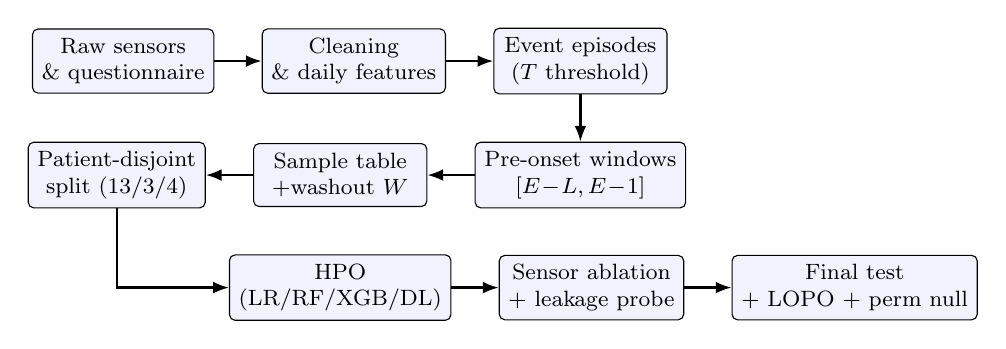
\begin{tikzpicture}[
  node distance=6mm,
  block/.style={draw,rounded corners=2pt,minimum height=8mm,
                minimum width=22mm,align=center,font=\footnotesize,
                fill=blue!5},
  arr/.style ={-{Latex[length=2mm]},thick}]
  \node[block] (a) {Raw sensors\\ \& questionnaire};
  \node[block,right=of a] (b) {Cleaning\\ \& daily features};
  \node[block,right=of b] (c) {Event episodes\\ ($T$ threshold)};
  \node[block,below=of c] (d) {Pre-onset windows\\ $[E\!-\!L,E\!-\!1]$};
  \node[block,left=of d] (e) {Sample table\\ +washout $W$};
  \node[block,left=of e] (f) {Patient-disjoint\\ split (13/3/4)};
  \node[block,below=of e] (g) {HPO\\ (LR/RF/XGB/DL)};
  \node[block,right=of g] (h) {Sensor ablation\\ + leakage probe};
  \node[block,right=of h] (i) {Final test\\ + LOPO + perm null};
  \draw[arr] (a)--(b); \draw[arr] (b)--(c); \draw[arr] (c)--(d);
  \draw[arr] (d)--(e); \draw[arr] (e)--(f);
  \draw[arr] (f) |- (g); \draw[arr] (g)--(h); \draw[arr] (h)--(i);
\end{tikzpicture}
\caption{End-to-end pipeline for the pre-onset anticipation task.}
\label{fig:pipeline}
\end{figure}

\subsection{Feature pipeline}

For each sample row with anchor day~$a$, per-day feature tables of
each selected sensor source are aggregated over $[a-L,\,a-1]$ using
mean / std / min / max / slope / last-value / count summaries and
merged with the patient-static descriptors.  At $L=14$ the
all-sensor table contains $427$ columns; the four single-modality
subsets used for ablation contain $216$ (smartwatch only),
$86$ (smartinhaler only), and the leave-one-out subsets reduce
the all-sensor count to $270$, $400$, and $355$ when smartwatch,
smartinhaler, and peak-flow respectively are removed.  Appendix~%
\ref{app:features} reports per-modality contributions.
Deep-learning models consume the underlying $L\times D$ daily
matrix directly rather than the aggregated table.

\subsection{Models}

\paragraph{Tabular baselines.}
Logistic regression (LR), random forest (RF), and gradient-boosted
trees (XGBoost) over the engineered feature table.

\paragraph{Deep-learning families.}
Four sequence-model families with comparable parameter budgets
(${\sim}24$k--$70$k):
\begin{itemize}[nosep,leftmargin=*]
  \item \textbf{Vanilla RNN}: two-layer Elman RNN, hidden dim 64,
        $\tanh$, dropout 0.2.
  \item \textbf{LSTM}: two-layer LSTM, hidden dim 64, dropout 0.2.
  \item \textbf{GRU}: two-layer GRU, hidden dim 64, dropout 0.2.
  \item \textbf{CNN}: three 1D convolutional blocks, kernel 3, ReLU,
        global average pooling.
\end{itemize}
All deep models are trained with Adam, BCE-with-logits with a
positive-class up-weight, batch size 64, and early stopping on
validation loss (patience~5, max 30~epochs).

% ==========================================================================
\section{Experimental Setup}\label{sec:setup}
% ==========================================================================

\subsection{Patient-disjoint split}

A single deterministic split is produced from the 18~unique
\texttt{user\_key}s under \texttt{np.random.default\_rng(seed=42)} and
reused at every downstream stage.

\begin{table}[H]
\centering
\caption{Fixed 13~/~3~/~4 patient-disjoint split.}
\label{tab:split}
\small
\begin{tabular}{lcl}
\toprule
\textbf{Fold} & \textbf{Size} & \textbf{User keys} \\
\midrule
Train & 13 & 939, 294, 113, 808, 343, 562, 917, 278,\\
      &    & 328, 867, 190, 701, 454 \\
Val   &  3 & 625, 514, 398 \\
Test  &  4 & 764, 473, 702, 447 \\
\bottomrule
\end{tabular}
\end{table}

The split is defined over \texttt{user\_key}s, not over samples;
several patients have no eligible labelled rows at high washout.
For example, at $(T=4,L=14,W=7)$ only $11$ of the $13$ training
patients contribute at least one sample to the training fold; the
remaining two have no stable-week anchor that survives the washout
filter.  Validation and test patient counts are not affected at
the cells reported in Section~\ref{sec:results-test}.

\subsection{Hyperparameter optimisation}

HPO covers $8$~LR grids, $24$~RF grids, $32$~XGBoost grids, and a
small DL architecture grid per cell, scored on validation \prauc{}.
One winner is selected per (cell, algorithm) triple.  Test rows
remain untouched during HPO.

\subsection{Multi-seed protocol}

For each deep-learning family and the winning $(T,L,W)$ cell, training
is repeated for 5~seeds $\{42,43,44,45,46\}$ on the same train/val/%
test patient split.  The only sources of variation across seeds are
weight initialisation, mini-batch ordering, and dropout sampling.

\subsection{Sensor ablation and label-leakage probe}

Each cell-winner is refit on nine sensor subsets (all,
four singletons, four leave-one-out) with hyperparameters locked from
HPO, yielding $9\times 27\times 3 = 729$~refits.  A 5-shuffle
label-permutation probe across all 81~configurations bounds the
ceiling under truly random labels.

\subsection{LOPO and patient-level permutation null}\label{sec:setup-lopo}

For each of the 18~patients $p$, the locked configuration is trained
on the other 17~and evaluated on $p$.  Per-patient
$\rocauc{}_p,\,\prauc{}_p$ are reported, and predictions are pooled
across folds for a global \rocauc{}/\prauc{}.  For each of $K=200$
permutations $\sigma$ of the 18~user keys, every patient's label
block is replaced by another patient's positional label block, and
the full LOPO is re-run.  The $p$-value is the fraction of permuted
pooled \rocauc{}s at least as large as the real value, with the
standard $+1$ smoother.

\subsection{Data-leakage prevention}\label{sec:setup-leakage}

Because leakage on small longitudinal cohorts can inflate scores by
an order of magnitude, the following controls are enforced uniformly
across all experiments:

\begin{itemize}[nosep,leftmargin=*]
  \item \textbf{Patient-disjoint splits before any tuning.}  The
        13/3/4 split (Table~\ref{tab:split}) is drawn from
        \texttt{user\_key}s once and frozen before HPO begins; no
        \texttt{user\_key} appears in more than one fold.
  \item \textbf{HPO scoped to train+val.}  Every grid search scores
        candidates on validation \prauc{} only.  Test predictions are
        never read during HPO or sensor ablation.
  \item \textbf{Train-only operating-point selection.}  The decision
        threshold $\tau^{\star}$ for $F_1$ reporting is selected on
        training predictions exclusively; validation and test
        predictions are never used for thresholding.
  \item \textbf{Post-onset washout.}  A washout window $W$ removes
        post-event days from the negative pool so that recovery-phase
        physiology does not contaminate the ``stable'' class.
  \item \textbf{Single test touch.}  The four-patient test fold is
        evaluated once per HPO winner, after the configuration is
        locked.  No iterative model selection is performed against
        test scores.
  \item \textbf{Patient-level permutation null.}  The LOPO null
        permutes user keys in blocks rather than rows, preventing
        spurious chance scores from per-patient label
        autocorrelation.
  \item \textbf{Label-permutation probe.}  A 5-shuffle row-level
        label permutation across all 81~configurations bounds the
        validation ceiling under truly random labels.
\end{itemize}

\subsection{Metrics, hardware, software}

We report \rocauc{} (rank-based), \prauc{} (more informative under
the ${\sim}4\%$ class prevalence of the reformulated task), Brier
score (calibration), and $F_1$ at a train-only-derived threshold
$\tau^{\star}$.  Under severe class imbalance, a random ranker has
expected \prauc{} approximately equal to the positive prevalence
($\approx 0.04$ here), so \prauc{} values must be compared against
that prevalence baseline rather than against $0.5$.  All experiments run on a single workstation
(Intel CPU, no GPU acceleration required).  Implementation uses
Python~3.12, \texttt{scikit-learn} 1.4, \texttt{xgboost} 2.0, and
\texttt{PyTorch} 2.4.  Bootstrap confidence intervals use 2000
resamples of the test predictions.

% ==========================================================================
\section{Results}\label{sec:results}
% ==========================================================================

\subsection{Original day-level baseline (pre-reformulation)}\label{sec:results-baseline}

Table~\ref{tab:phase1} reports the \emph{original} day-level
baseline that motivated the reformulation described in
Section~\ref{sec:method}.  This setup used 24-hour windows with a
1-hour stride, smartwatch features only, and a week-level
propagated label; it is the same configuration whose three
protocol-level weaknesses are enumerated in Section~\ref{sec:method}
(within-patient temporal redundancy, coarse week-level label, and
single-seed deep-learning evaluation).  The numbers are reproduced
here unchanged from the project's interim baseline run -- not
re-executed after the leakage controls and label redesign were
introduced -- and are therefore \emph{not} directly comparable to
the reformulated-task results in later subsections.  Three
specific defects of that interim run motivated the redesign:
(a)~the weekly worsening label was propagated to all
$\sim$168~minute-level windows of every positive week, so adjacent
windows (with $95.8\%$ shared data) inflated the effective
positive count and rewarded patient-identity rather than
onset-anticipation; (b)~the multimodal variant of this run
included the daily-questionnaire worsening score as a feature
alongside its use in label construction, which produced an
optimistic-looking $\rocauc{}\approx 0.93$ on the same split
before that feature was excluded as a label proxy; and
(c)~deep-learning models were trained on a single seed, which
Section~\ref{sec:results-multiseed} shows is uninformative on
this cohort.  Table~\ref{tab:phase1} is retained as the
``before'' picture that motivates the rest of the report.

A diagnostic 5-fold GroupKFold cross-validation of the Random
Forest on the same pre-reformulation feature table yielded mean
\rocauc{}~$=~0.611\pm 0.226$ with per-fold range $[0.37,\,0.91]$,
which provided the first quantitative evidence that inter-patient
variance dominates this task and prompted the redesign.

\begin{table}[H]
\centering
\caption{Original (pre-reformulation) day-level baseline on a
single 25\%-patient-wise split with week-propagated labels.  These
numbers are retained for context only and should not be read as a
fair comparator for the reformulated-task results in
Table~\ref{tab:onset-headline}; see Section~\ref{sec:results-baseline}
for the precise caveat.}
\label{tab:phase1}
\small
\begin{tabular}{lcccccc}
\toprule
\textbf{Model} & \textbf{Prec} & \textbf{Rec} & \textbf{F1} &
\textbf{\rocauc{}} & \textbf{\prauc{}} & \textbf{Brier} \\
\midrule
GRU (2-layer)       & 0.481 & 0.918 & 0.632 & 0.717 & 0.773 & 0.225 \\
Ensemble (60\%~GRU) & 0.823 & 0.549 & 0.659 & 0.653 & 0.762 & 0.221 \\
Random Forest       & 0.854 & 0.402 & 0.547 & 0.633 & 0.724 & 0.254 \\
XGBoost             & 0.812 & 0.255 & 0.388 & 0.581 & 0.654 & 0.312 \\
Logistic Reg.       & 0.523 & 0.588 & 0.554 & 0.578 & 0.658 & 0.313 \\
CNN (3-layer)       & 0.475 & 0.694 & 0.564 & 0.520 & 0.530 & 0.320 \\
\bottomrule
\end{tabular}
\end{table}

\subsection{Multi-seed deep-learning evaluation}\label{sec:results-multiseed}

Table~\ref{tab:rnn-multiseed} reports the test \rocauc{} of the
HPO-winning RNN at $(T=3,L=14,W=14)$ across five seeds on the
\emph{same} 4-patient test fold; everything other than the random
seed is identical between runs.

\begin{table}[H]
\centering
\caption{RNN multi-seed test \rocauc{} on the fixed test fold.}
\label{tab:rnn-multiseed}
\small
\begin{tabular}{rc}
\toprule
\textbf{Seed} & \textbf{Test \rocauc{}} \\
\midrule
42 & 0.900 \\
43 & 0.920 \\
44 & 0.387 \\
45 & 0.654 \\
46 & 0.381 \\
\midrule
Mean $\pm$ std & $0.648 \pm 0.263$ \\
Range          & $[0.381,\,0.920]$ \\
\bottomrule
\end{tabular}
\end{table}

The within-seed range of $\Delta\rocauc=0.54$ exceeds the spread
between any two model families in Table~\ref{tab:phase1}.
Single-seed reporting on this cohort therefore samples from a
heavy-tailed distribution and is not a reliable summary of model
behaviour.

\subsection{Sample population and HPO winners}\label{sec:results-hpo}

The number of pre-onset positive samples is bounded by the small
number of distinct event episodes per patient.  At $L=14$, each of
the three threshold settings produces 53--55 positives across the
full cohort; positive rates fall in the range $4.3$--$4.9\%$.

\begin{table}[H]
\centering
\caption{Sample counts at $L=14$ across all 18~patients.}
\label{tab:onset-counts}
\small
\begin{tabular}{ccccccc}
\toprule
$T$ & $L$ & $W$ & \textbf{Pos.} & \textbf{Neg.} &
\textbf{Total} & \textbf{Pos.~rate} \\
\midrule
2 & 14 & 0  & 54 & 1191 & 1245 & 4.34\% \\
2 & 14 & 7  & 54 & 1130 & 1184 & 4.56\% \\
2 & 14 & 14 & 54 & 1067 & 1121 & 4.82\% \\
3 & 14 & 0  & 53 & 1191 & 1244 & 4.26\% \\
3 & 14 & 7  & 53 & 1134 & 1187 & 4.47\% \\
3 & 14 & 14 & 53 & 1071 & 1124 & 4.72\% \\
4 & 14 & 0  & 55 & 1191 & 1246 & 4.41\% \\
4 & 14 & 7  & 55 & 1139 & 1194 & 4.61\% \\
4 & 14 & 14 & 55 & 1076 & 1131 & 4.86\% \\
\bottomrule
\end{tabular}
\end{table}

At the headline RF cell $(T=4,L=14,W=7)$ the four test patients
contribute 4~positives out of 339~test samples ($1.18\%$); at the
headline XGB-inhaler cell $(T=4,L=14,W=14)$, 4 of 325 ($1.23\%$).
HPO winners are summarised in Table~\ref{tab:hpo-winners}.

\begin{table*}[t]
\centering
\caption{HPO winners feeding the test and LOPO tables.}
\label{tab:hpo-winners}
\small
\begin{tabular}{lcccll cc}
\toprule
\textbf{Algo} & $T$ & $L$ & $W$ & \textbf{Sensor subset} &
\textbf{Winning hyperparameters} & \textbf{Val \prauc{}} &
\textbf{Test \rocauc{}} \\
\midrule
RF  & 4 & 14 & 7  & all (4 modalities)  & cw=balanced; $n$=200; depth=None; leaf=1 & 0.250 & 0.879 \\
RF  & 4 & 14 & 14 & all                 & cw=balanced; $n$=500; depth=6; leaf=1    & 0.015 & 0.650 \\
XGB & 4 & 14 & 0  & all                 & $n$=200; depth=6; lr=0.05; subs=0.7      & 0.034 & 0.759 \\
XGB & 4 & 14 & 14 & smartinhaler only   & $n$=200; depth=3; lr=0.1; subs=1.0       & 0.013 & 0.964 \\
RNN & 3 & 14 & 14 & all (daily tensor)  & hidden=64; layers=2; dropout=0.2         & 0.123 & $0.648 \pm 0.263$ \\
\bottomrule
\end{tabular}
\end{table*}

A 5-shuffle label-permutation probe across all 81~configurations
yields a pooled mean validation \rocauc{} under permuted labels of
$0.5046$ (95\% empirical interval $\approx[0.25,0.75]$), consistent
with no label-side leakage.

\subsection{Held-out test results}\label{sec:results-test}

\begin{table}[H]
\centering
\caption{Held-out test results on 4~patients; 95\% CIs are bootstrap
with 2000~resamples.}
\label{tab:onset-headline}
\small
\begin{tabular}{lcccc}
\toprule
\textbf{Config} & \textbf{\rocauc{}} & \textbf{\prauc{}} &
$F_1^{\,\tau^{\star}}$ & \textbf{Brier} \\
\midrule
RF -- all sensors        & 0.879 [0.65, 1.00] & 0.327 & 0.000 & 0.027 \\
XGB -- all sensors       & 0.759 [0.63, 1.00] & 0.269 & 0.400 & 0.019 \\
XGB -- smartinhaler only & \textbf{0.964}     & \textbf{0.164} & \textbf{0.136} & 0.168 \\
RNN -- multi-seed        & $0.648\pm 0.263$   & ---   & ---   & --- \\
\bottomrule
\end{tabular}
\end{table}

Three observations frame these results.  First, the RF tuned-$F_1$
is $0$ at the default $0.5$ cutoff because the model ranks the four
test positives correctly but never crosses that cutoff -- a
strong-ranking but uncalibrated decision boundary on a 4-positive
test set.  Second, the XGB-inhaler \prauc{} of $0.164$ is roughly
$20\times$ the prevalence baseline of $\approx 0.04$.  Third, the
RNN multi-seed spread shows that any single-seed deep-learning
headline on this cohort should be interpreted as a draw from the
seed distribution in Table~\ref{tab:rnn-multiseed}, not as a stable
point estimate.

\paragraph{Ranking versus alarm behaviour.}
The disparity between \rocauc{} and threshold-based metrics in
Table~\ref{tab:onset-headline} is a generic property of
rank-AUC under extreme imbalance: with four positives among 339
test samples, even random scoring places half of the positives in
the top 50\% of the ranking, so a \rocauc{} of $0.879$ is
compatible with a wide range of operating-point behaviours.  In
particular, the RF assigns probabilities $<0.5$ to all four
positives -- they are ranked above the negatives but lie below the
default decision boundary -- so $F_1=0$.  An accurate ranker is
not the same object as a deployable alarm system; the latter
requires a stable, calibrated threshold whose stability cannot be
established on a 4-positive fold.  Bootstrap CIs in this regime
should be read as descriptive bands rather than as inferential
intervals.

\begin{table}[H]
\centering
\caption{Big-picture summary of the headline results.}
\label{tab:summary}
\small
\begin{tabular}{lc}
\toprule
\textbf{Evaluation} & \textbf{Result} \\
\midrule
Day-level baseline (RF, GroupKFold, \emph{pre-fix}) & $0.611 \pm 0.226$ \\
RNN multi-seed on fixed test fold          & $0.648 \pm 0.263$ \\
Best held-out test (XGB, smartinhaler)     & $0.964$ \\
Best held-out test (RF, all sensors)       & $0.879$ \\
LOPO pooled (XGB, smartinhaler)            & $0.619$ ($p=0.22$) \\
LOPO pooled (RF, all sensors)              & $0.354$ ($p=0.40$) \\
\bottomrule
\end{tabular}
\end{table}

\subsection{Sensor ablation}\label{sec:results-ablation}

Across the 27-cell grid, smartinhaler-only features dominate the
sensor ablation at every threshold.  The best smartinhaler-only
configuration ($T=4,L=14,W=14$) yields the highest test \rocauc{}
in the entire grid, exceeding every all-sensor counterpart.  This
is consistent with Lugogo et~al.~\cite{lugogo2022}, in which
connected-inhaler signals alone produced clinically meaningful
discrimination.

\subsection{LOPO cross-patient evaluation}\label{sec:results-lopo}

The two strongest configurations from Table~\ref{tab:onset-headline}
were re-evaluated under leave-one-patient-out across all
18~patients, with a 200-permutation patient-level null
(Section~\ref{sec:setup-lopo}).

\begin{table}[H]
\centering
\caption{LOPO results across all 18~patients.}
\label{tab:lopo}
\small
\begin{tabular}{lccc}
\toprule
\textbf{Config} & \textbf{Held-out test} &
\textbf{Pooled \rocauc{}} & \textbf{Per-patient \rocauc{}} \\
\midrule
RF -- all sensors        & 0.879 & \textbf{0.354} &
$0.641 \pm 0.255$ \\
XGB -- smartinhaler only & 0.964 & \textbf{0.619} &
$0.521 \pm 0.293$ \\
\bottomrule
\end{tabular}
\end{table}

\begin{table}[H]
\centering
\caption{Patient-level permutation null at $K=200$.}
\label{tab:lopo-null}
\small
\begin{tabular}{lccccc}
\toprule
\textbf{Config} & \textbf{Real} & \textbf{Null mean} &
$q_{05}$ & $q_{95}$ & \textbf{$p$} \\
\midrule
RF -- all sensors        & 0.354 & 0.342 & 0.125 & 0.664 & 0.40 \\
XGB -- smartinhaler only & 0.619 & 0.440 & 0.135 & 0.807 & 0.22 \\
\bottomrule
\end{tabular}
\end{table}

Pooled LOPO \rocauc{} of the all-sensor RF is $0.354$, with a
permutation $p$-value of $0.40$; the inhaler-only XGB is $0.619$,
with $p=0.22$.  Both real values sit comfortably inside the
$[q_{05},q_{95}]$ envelope of the null.  Under the patient-level
null hypothesis, neither configuration produces statistically
distinguishable cross-patient discrimination at $\alpha=0.05$.

\subsection{Coverage-aware stratification}\label{sec:results-coverage}

Because per-patient HR missingness ranges from $18.06\%$ to
$61.57\%$, the LOPO collapse could in principle be driven by
patients with very sparse coverage.  We stratified the per-patient
RF-all-sensors LOPO \rocauc{} by the held-out patient's
HR-missingness tier, restricted to the 9 folds with defined
\rocauc{}.  The remaining 9~folds have an undefined per-patient
\rocauc{} because the held-out patient's evaluation block contains
only one class (no pre-onset positive within the patient's record,
or no eligible stable negative under the active washout); in such
folds \rocauc{} is mathematically undefined and the patient is
excluded from the per-patient mean.  Pooled \rocauc{} is still
computed over all 18~folds because pooling concatenates raw scores
before the AUC is taken.

\begin{table}[H]
\centering
\caption{RF LOPO \rocauc{} stratified by held-out HR missingness.}
\label{tab:lopo-coverage}
\small
\begin{tabular}{lcc}
\toprule
\textbf{Tier} & \textbf{Patients} & \textbf{Mean \rocauc{}} \\
\midrule
Low ($<25\%$)   & 113, 294, 343, 447, 701, 939 & 0.555 \\
Mid (25--40\%)  & 625                          & 1.000 \\
High ($>40\%$)  & 473, 808                     & 0.720 \\
\bottomrule
\end{tabular}
\end{table}

High-missingness patients score higher, not lower; the LOPO
collapse is not parsimoniously explained as a coverage artefact on
this cohort.  The stratification is itself fragile (two patients in
the high tier) and indicative rather than conclusive.

% ==========================================================================
\section{Discussion}\label{sec:discussion}
% ==========================================================================

\subsection{Findings}

\paragraph{Reformulated task.}
Anchoring positives on the day before each onset removes the
weekly-label propagation problem of the day-level baseline.  The
label-leakage probe (pooled permuted \rocauc{} $=0.5046$) confirms
that the new sample construction does not introduce inadvertent
label-side leakage.

\paragraph{Modality contribution.}
Smartinhaler-only features produce the highest \rocauc{} of any
configuration in the grid on the held-out fold ($0.964$) and the
highest pooled LOPO \rocauc{} ($0.619$ vs.\ $0.354$ for the
all-sensor RF), although neither result is significant under the
patient-level null.  This is consistent with prior work showing
strong discrimination from connected-inhaler signals
alone~\cite{lugogo2022}.

\paragraph{Reporting protocol vs.\ architecture.}
The variance attributable to the random seed in
Table~\ref{tab:rnn-multiseed} ($\sigma=0.26$) and to the choice of
LOPO held-out patient in Table~\ref{tab:lopo} ($\sigma\approx 0.26$)
both exceed the gap between any two model families on the held-out
fold.  On this cohort, the choice of reporting protocol affects
the headline more than the choice of architecture.

\subsection{What this work does not establish}

\begin{itemize}[nosep,leftmargin=*]
  \item \textbf{Cross-patient generalisation.}  No tabular or
        deep-learning configuration in this report achieves a
        cross-patient effect size that rejects the patient-permutation
        null at $\alpha=0.05$.
  \item \textbf{Clinical operating-point selection.}  $F_1$-tuned
        thresholds were derived from training data only and were not
        stability-tested across patient folds.
  \item \textbf{Modality-specific causal claims.}  Smartinhaler
        dominance in the ablation is consistent with prior literature
        but cannot be attributed to a specific behavioural mechanism
        at $n=18$.
\end{itemize}

\subsection{Why LOPO collapses}

The gap between the held-out test fold ($\rocauc{}\in[0.76,0.96]$)
and pooled LOPO ($\rocauc{}\in[0.35,0.62]$) is large enough to
require mechanistic explanation rather than a generic ``small
cohort'' label.  Four factors are likely jointly responsible.
(i)~\emph{Inter-patient heterogeneity}: asthma phenotypes (allergic,
eosinophilic, exercise-induced) produce qualitatively different
physiological signatures, so a decision boundary fit on
17~patients is required to extrapolate across phenotypes when
evaluated on the 18th.  (ii)~\emph{Wearable-adherence variation}:
per-user HR missingness ranges from $18\%$ to $62\%$ and inhaler
actuation logging is event-driven rather than continuous, so the
effective feature dimension is patient-dependent.
(iii)~\emph{Sparse event counts}: each patient contributes only a
handful of episodes, so any one held-out patient can shift pooled
\rocauc{} by tens of points.  (iv)~\emph{Absence of personalised
baselines}: the models learn a population-level decision
boundary, whereas exacerbation onset is most plausibly defined as
a deviation from each patient's own stable distribution.  Cohort
size is the binding constraint, but the LOPO collapse is a
composite of these four mechanisms rather than sample size alone.

\subsection{Implications}

The variance patterns documented here -- 5-seed test
\rocauc{}~$=0.65\pm 0.26$ on a fixed split and LOPO pooled
\rocauc{} of $0.35$--$0.62$ -- quantify a stability concern that is
known qualitatively in the wearable-asthma literature~%
\cite{molfino2024,dehond2022,cokorudy2024}.  Three practical
recommendations follow: when $n_{\text{test}}\leq 5$, headline
results should be reported alongside an LOPO companion; recurrent
models on cohorts of this size require multi-seed reporting; and a
patient-block permutation null is more diagnostic than a row-level
feature shuffle, because the latter can be inflated by per-patient
confounding.

% ==========================================================================
\section{Limitations}\label{sec:limits}
% ==========================================================================

\paragraph{Cohort size.}
The binding limitation is $n=18$ usable patients.  At this scale,
the per-patient within-class variance is comparable to the
between-class effect, and even a perfectly clean protocol cannot
produce significant generalisation evidence.

\paragraph{Single-study cohort.}
AAMOS-00 is a single UK-based study; external validation on at
least one independent multimodal cohort is required before any
deployment-style claim.

\paragraph{Coarse questionnaire ground truth.}
The weekly worsening score is more reliable than self-reported
daily symptoms but coarser than clinician-documented events.  Some
of the per-patient \rocauc{} variance is likely attributable to
questionnaire-completion behaviour rather than to physiological
signal.

\paragraph{No deep-learning cross-patient evaluation.}
LOPO with patient-permutation null was applied only to the two
strongest tabular configurations.  The multi-seed evidence in
Table~\ref{tab:rnn-multiseed} establishes reporting stability for
recurrent models but does not test cross-patient transfer; an
18-fold $\times$ 5-seed LOPO over the RNN, LSTM, GRU, and CNN
families would be needed for that.  Consequently, the
generalisation of recurrent models on this cohort remains
untested.

\paragraph{No deployment-grade calibration.}
We report Brier scores but do not perform Platt or isotonic
recalibration: the test set is too small for stable calibration
learning, and the LOPO instability of the predictors would
propagate into any post-hoc calibration map.

\paragraph{Bootstrap confidence intervals.}
Because the held-out fold contains only four positive samples,
bootstrap 95\% intervals on test \rocauc{} should be interpreted
cautiously: resampling 4 positives produces a high-variance
empirical distribution, and the resulting bands describe
resampling variability on a fixed fold rather than cross-patient
uncertainty, which the LOPO analysis estimates instead.

\paragraph{Ethics, privacy, and clinical scope.}
Wearable and inhaler streams are intimate behavioural signals;
any deployment-style use must satisfy informed-consent, secure
storage, and minimum-necessary-data constraints beyond what a
research cohort like AAMOS-00 requires.  False alarms in an early
warning system have non-trivial costs (alarm fatigue, unnecessary
rescue-medication use, anxiety), and missed warnings have
clinical costs.  The pipeline reported here is a research
prototype: it is not calibrated for deployment, was not evaluated
for subgroup fairness, and would require physician oversight,
prospective validation, and regulatory review before any
patient-facing use.

% ==========================================================================
\section{Conclusion and Future Work}\label{sec:conclusion}
% ==========================================================================

We presented an end-to-end pipeline for early warning of asthma
exacerbations from multimodal wearable data, reformulating the
prediction task as event-episode pre-onset anticipation with
patient-disjoint splits at every stage.  On a held-out four-patient
test fold the strongest configurations achieved \rocauc{}
of~$0.879$ (RF, all sensors) and $0.964$ (XGB,
smartinhaler-only).  Under leave-one-patient-out across the full
18-patient cohort, pooled \rocauc{} dropped to $0.354$ and $0.619$
respectively, and a 200-permutation patient-level null could not
distinguish either from chance ($p=0.40$ and $p=0.22$).  At
$n=18$, headline scores on a 4-patient split should be interpreted
together with the LOPO companion; the present results indicate
that cross-patient generalisation in this cohort is bounded
primarily by sample size rather than by modelling capacity.
Even imperfect anticipation, once validated at scale, could help
trigger earlier self-management interventions (inhaler adherence
checks, peak-flow prompts, clinician contact) before clinical
deterioration sets in -- the clinical motivation that justifies
continued investment in this prediction task despite the present
statistical limits.

Future work should prioritise: (i) replication on a larger
multimodal cohort ($n\geq 50$) where the patient-permutation null
can be rejected at $\alpha=0.05$ for a clinically meaningful
effect size; (ii) inhaler-centric modelling with denser
instrumentation, including time-since-last-use kernels and
circadian decompositions; (iii) personalised per-patient baselines
that model departures from each patient's stable distribution
rather than a population-level decision boundary; (iv) multi-horizon
evaluation across $\{3,7,14\}$-day pre-onset windows with shared
backbone weights; and (v) self-supervised pretraining on adjacent
generic-wearable corpora before fine-tuning on AAMOS-00.

% ==========================================================================
\bibliographystyle{unsrtnat}
\begin{thebibliography}{20}

\bibitem{who2024}
World Health Organization, ``Asthma,'' Fact Sheet, May 6, 2024.

\bibitem{bourdin2019}
A.~Bourdin et~al., ``ERS/EAACI statement on severe exacerbations in
asthma,'' \emph{European Respiratory Journal}, vol.~54, no.~3, 2019.

\bibitem{nurmagambetov2018}
T.~Nurmagambetov, R.~Kuwahara, and P.~Garbe, ``The economic burden of
asthma in the United States, 2008--2013,'' \emph{Annals of the American
Thoracic Society}, 2018.

\bibitem{pinnock2015}
H.~Pinnock, ``Supported self-management for asthma,''
\emph{Breathe (ERS)}, 2015.

\bibitem{cokorudy2024}
B.~Cokorudy, K.~C.~H.~Tsang, S.~A.~Shah, and A.~Sheikh, ``Digital
markers of asthma exacerbations: a systematic review,''
\emph{npj Digital Medicine}, vol.~7, Art.~no.~84, 2024.

\bibitem{taylor2020}
L.~Taylor, M.~Ding, J.~Wilkinson, and H.~Pinnock, ``Wearable vital
signs monitoring for patients with chronic respiratory disease: a
scoping review,'' \emph{npj Digital Medicine}, vol.~3, Art.~no.~155,
2020.

\bibitem{cho2021}
J.~Cho, J.~Kim, and S.~Park, ``Wearable health data quality and
missingness: a systematic review of methods,'' \emph{Journal of
Medical Internet Research}, vol.~23, no.~10, 2021.

\bibitem{molfino2024}
N.~A.~Molfino and G.~Turcatel, ``Machine learning approaches to
predict asthma exacerbations: a narrative review,'' \emph{Respiratory
Research}, vol.~25, Art.~no.~129, 2024.

\bibitem{dehond2022}
A.~A.~H.~de~Hond et~al., ``Machine learning did not beat logistic
regression in time series prediction for severe asthma exacerbations,''
\emph{Scientific Reports}, vol.~12, Art.~no.~20363, 2022.

\bibitem{lugogo2022}
N.~L.~Lugogo et~al., ``A predictive machine learning tool for asthma
exacerbations using an electronic inhaler with integrated sensors,''
\emph{Journal of Asthma and Allergy}, 2022.

\bibitem{tsang2023}
K.~C.~H.~Tsang et~al., ``Home monitoring with connected mobile devices
for asthma attack prediction with machine learning,''
\emph{Scientific Data}, 2023.

\bibitem{chan2024}
A.~H.~Y.~Chan et~al., ``DIGIPREDICT: physiological, behavioural and
environmental predictors of asthma attacks---study protocol,''
\emph{BMJ Open Respiratory Research}, 2024.

\bibitem{datashare}
University of Edinburgh DataShare, ``AAMOS-00 dataset repository,''
CC~BY~4.0.

\bibitem{bai2018}
S.~Bai, J.~Z.~Kolter, and V.~Koltun, ``An empirical evaluation of
generic convolutional and recurrent networks for sequence modeling,''
\emph{arXiv preprint arXiv:1803.01271}, 2018.

\bibitem{ganaie2021}
M.~A.~Ganaie, M.~Hu, A.~K.~Malik, M.~Tanveer, and P.~N.~Suganthan,
``Ensemble deep learning: a review,'' \emph{Engineering Applications
of Artificial Intelligence}, vol.~115, Art.~no.~105151, 2022.

\end{thebibliography}

% ==========================================================================
\appendix
\section{Hyperparameter grids}\label{app:grids}
% ==========================================================================

\paragraph{Logistic regression (8 grids).}
$C\in\{0.01,0.1,1,10\}$;
\texttt{class\_weight}$\in\{\text{None},\text{balanced}\}$;
solver \texttt{liblinear}; penalty \texttt{l2}; max\_iter 1000.

\paragraph{Random forest (24 grids).}
\texttt{n\_estimators}$\in\{200,500\}$;
\texttt{max\_depth}$\in\{\text{None},6,12\}$;
\texttt{min\_samples\_leaf}$\in\{1,5\}$;
\texttt{class\_weight}$\in\{\text{None},\text{balanced}\}$;
\texttt{criterion}=\texttt{gini}.

\paragraph{XGBoost (32 grids).}
\texttt{n\_estimators}$\in\{200,500\}$;
\texttt{max\_depth}$\in\{3,6\}$;
\texttt{learning\_rate}$\in\{0.05,0.1\}$;
\texttt{subsample}$\in\{0.7,1.0\}$;
\texttt{colsample\_bytree}$\in\{0.7,1.0\}$;
\texttt{objective}=\texttt{binary:logistic};
\texttt{eval\_metric}=\texttt{aucpr};
\texttt{scale\_pos\_weight} $=N_{\text{neg}}/N_{\text{pos}}$ on the
training fold; \texttt{tree\_method}=\texttt{hist}.

\paragraph{Deep-learning families.}
For each of RNN, LSTM, GRU, CNN:
\texttt{hidden\_dim}$\in\{32,64\}$;
\texttt{num\_layers}$\in\{1,2\}$;
\texttt{dropout}$\in\{0.1,0.2\}$.
Optimizer Adam, learning rate $10^{-3}$, weight decay $10^{-4}$,
batch size 64.  Loss is BCE-with-logits with positive-class weight
$N_{\text{neg}}/N_{\text{pos}}$ on the training fold.  Early
stopping monitors validation loss with patience~5, maximum
30~epochs; the best-validation-loss checkpoint is restored before
test evaluation.

% ==========================================================================
\section{Feature inventory}\label{app:features}
% ==========================================================================

For each sensor source, per-day features are first computed from
minute-level streams, then aggregated over the lookback window
$[a-L,\,a-1]$ using the operators
$\{\text{mean},\text{std},\text{min},\text{max},\text{slope},
\text{last},\text{count}\}$.

\begin{table}[H]
\centering
\caption{Per-modality feature counts at $L=14$.}
\label{tab:features-app}
\small
\begin{tabular}{lcl}
\toprule
\textbf{Subset} & \textbf{Sensors retained} & \textbf{Dim.} \\
\midrule
All               & SW + SI + PF + ENV + static    & 427 \\
Smartwatch only   & SW + static                    & 216 \\
Smartinhaler only & SI + static                    &  86 \\
No smartwatch     & SI + PF + ENV + static         & 270 \\
No smartinhaler   & SW + PF + ENV + static         & 400 \\
No peak-flow      & SW + SI + ENV + static         & 355 \\
\bottomrule
\end{tabular}
\end{table}

The per-modality contributions implied by the leave-one-out
subsets are: smartwatch ${\approx}157$, smartinhaler
${\approx}27$, peak-flow ${\approx}72$, environment + static
${\approx}171$ columns.  Counts do not add to the
single-modality ``only'' rows because each modality-only subset
is padded with patient-static features.  All numbers above are
read directly from \texttt{n\_features} in the
\texttt{sensor\_ablation\_v2.csv} grid and from the HPO winners
in \texttt{tune\_tabular\_v2\_best.csv}.

\paragraph{Missingness handling.}
Minute-level HR values outside $[30,220]$~bpm are nulled; gaps
$\leq 5$~minutes are forward-filled, longer gaps left as NaN.  At
the daily-aggregate level, missing aggregates are imputed with the
training-fold per-feature median; an indicator column flags the
imputation.  Patient-static fields are one-hot encoded.

% ==========================================================================
\section{Compute and runtime}\label{app:compute}
% ==========================================================================

All experiments run on a single workstation (Intel CPU, 32~GB RAM,
no GPU).  Approximate wall-clock costs:

\begin{itemize}[nosep,leftmargin=*]
  \item Full 27-cell HPO over LR+RF+XGB across 9 sensor subsets:
        ${\sim}4$~hours.
  \item Per deep-learning family, 5-seed run on the winning cell:
        ${\sim}25$~minutes.
  \item 200-permutation LOPO null per configuration:
        ${\sim}90$~minutes.
\end{itemize}

Software: Python~3.12, \texttt{numpy} 1.26,
\texttt{scikit-learn} 1.4, \texttt{xgboost} 2.0,
\texttt{PyTorch} 2.4, \texttt{pandas} 2.2.  All random seeds and
the train/val/test split are fixed at
\texttt{numpy.random.default\_rng(seed=42)}.

\end{document}
